\section{Allele and genotype frequencies}

\subsection{Allele frequencies}
Consider a diploid autosomal locus segregating at two alleles ($A_1$ and $A_2$). Let $N_{11}$ and $N_{12}$ be the number of $A_1A_1$ homozygotes and $A_1A_2$ heterozygotes, respectively. Moreover, let $N$ be the total number of diploid individuals in the population. We can then define the relative frequencies of $A_1A_1$ and $A_1A_2$ genotypes as $f_{11} = N_{11}/N$ and $f_{12} = N_{12}/N$, respectively. The frequency of allele $A_1$ in the population is then given by
\begin{equation}
p = \frac{2 N_{11} + N_{12}}{2N} = f_{11} + \frac{1}{2} f_{12}. % Modified by Simon
\end{equation}
Note that this holds independently of Hardy--Weinberg proportions and equilibrium [see below]. The frequency of the alternate allele ($A_2$) is then just $q=1-p$.

\subsection{Hardy--Weinberg proportions}

Imagine a population mating at random with respect to genotypes, i.e.\
no inbreeding, no population structure, no sex differences in allele frequencies. The frequency of allele $A_1$ in the population at the time of reproduction is $p$. An $A_1A_1$ genotype is made by reaching out into our population and independently drawing two $A_1$ alelle gametes to form a zygote. Therefore, the probability that an individual is an $A_1A_1$ homozygote is $p^2$. This probability is also the expected frequency of the $A_1A_1$ homozygote in the population. The expected frequency of the three possible genotypes is
%\begin{table}[htp!]
\begin{center}
\begin{tabular}{|ccc|}
\hline
$f_{11}$ & $f_{12}$ & $f_{22}$ \\
\hline
$p^2$ & $2pq$ & $q^2$ \\
\hline
\end{tabular}\,.
\end{center}
%\caption{\textbf{Hardy Weinberg}} \label{table:HWE}
%\end{table}
Note that we only need to assume random mating with
respect to our alleles in order for these expected frequencies to hold,
as long at $p$ is the frequency of the $A_1$ allele in the population at
the time when gametes fuse.


%%%ADD A comment about WF sampling here!
%% Also add a question about Poisson offspring number.

\begin{figure}
\begin{center}
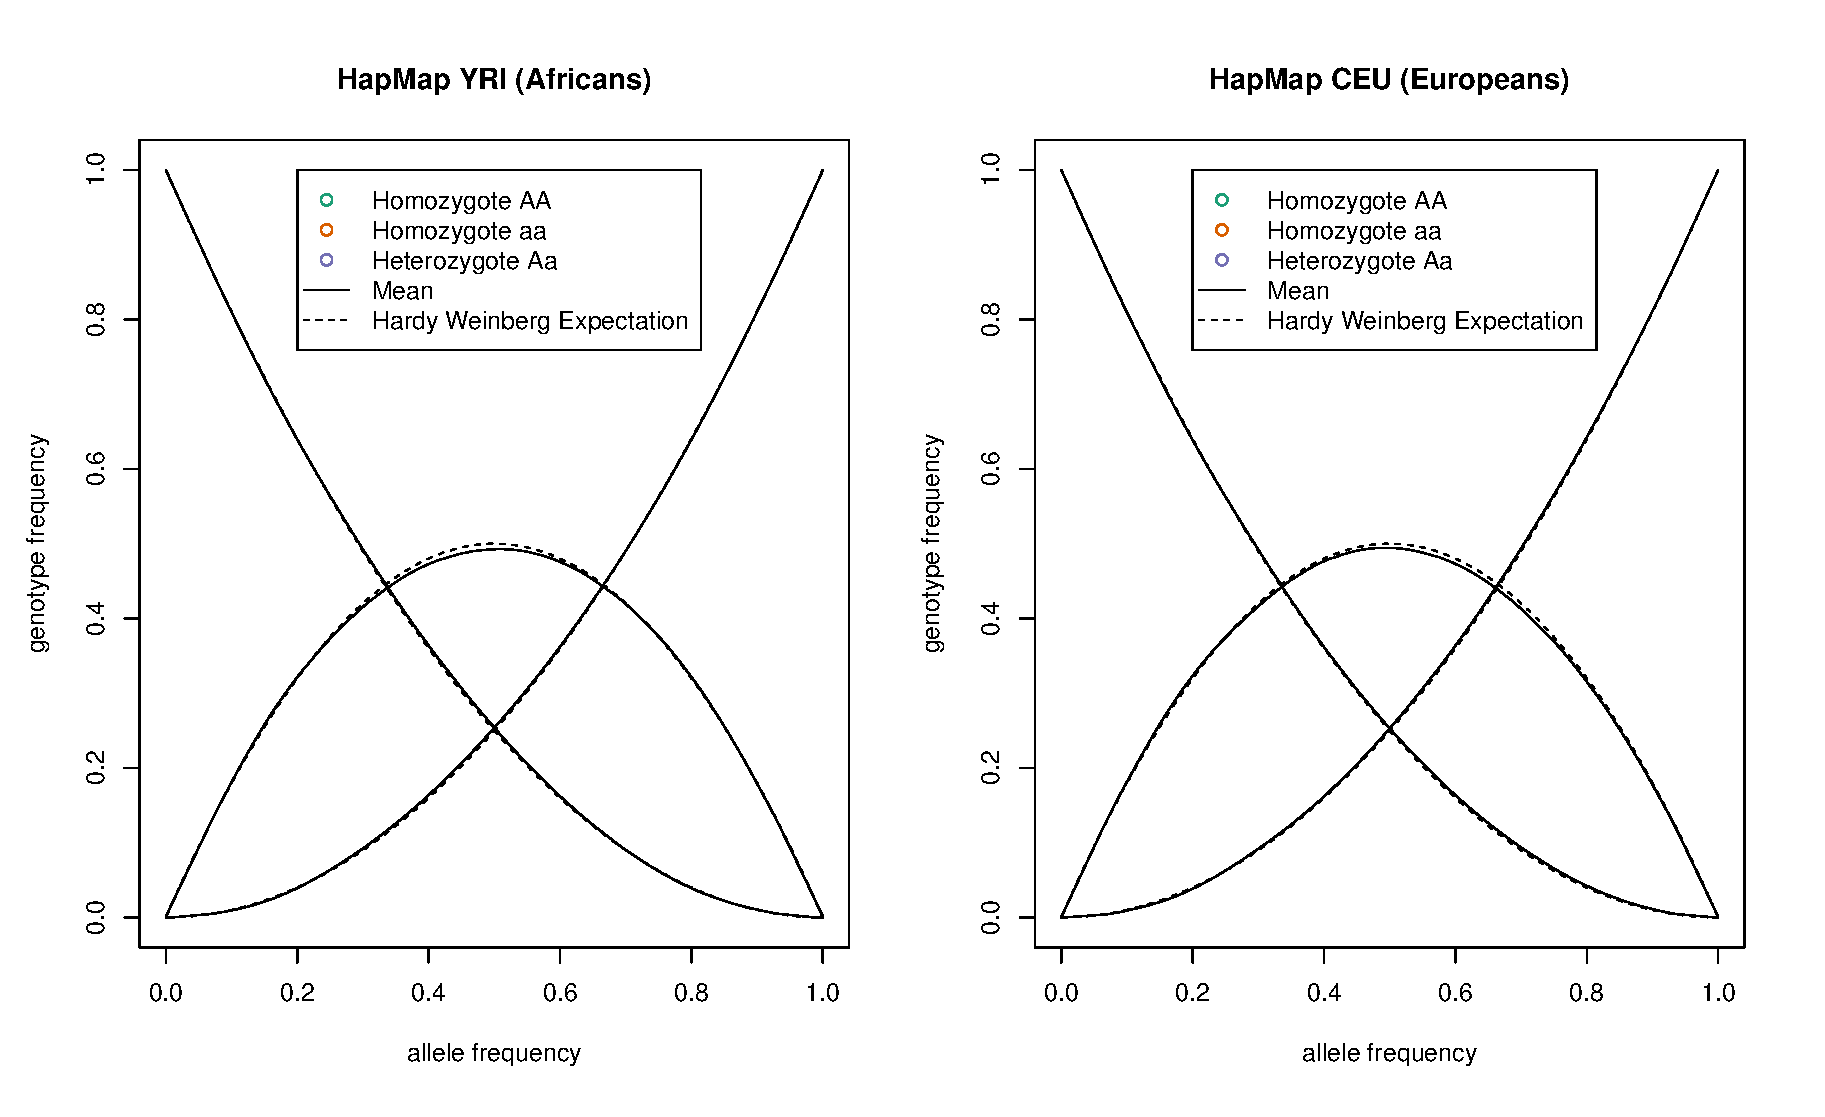
\includegraphics[width=0.8 \textwidth]{figures/CEU_YRI_separately_HWE.eps}
\end{center}
\end{figure}


\begin{figure}
\begin{center}
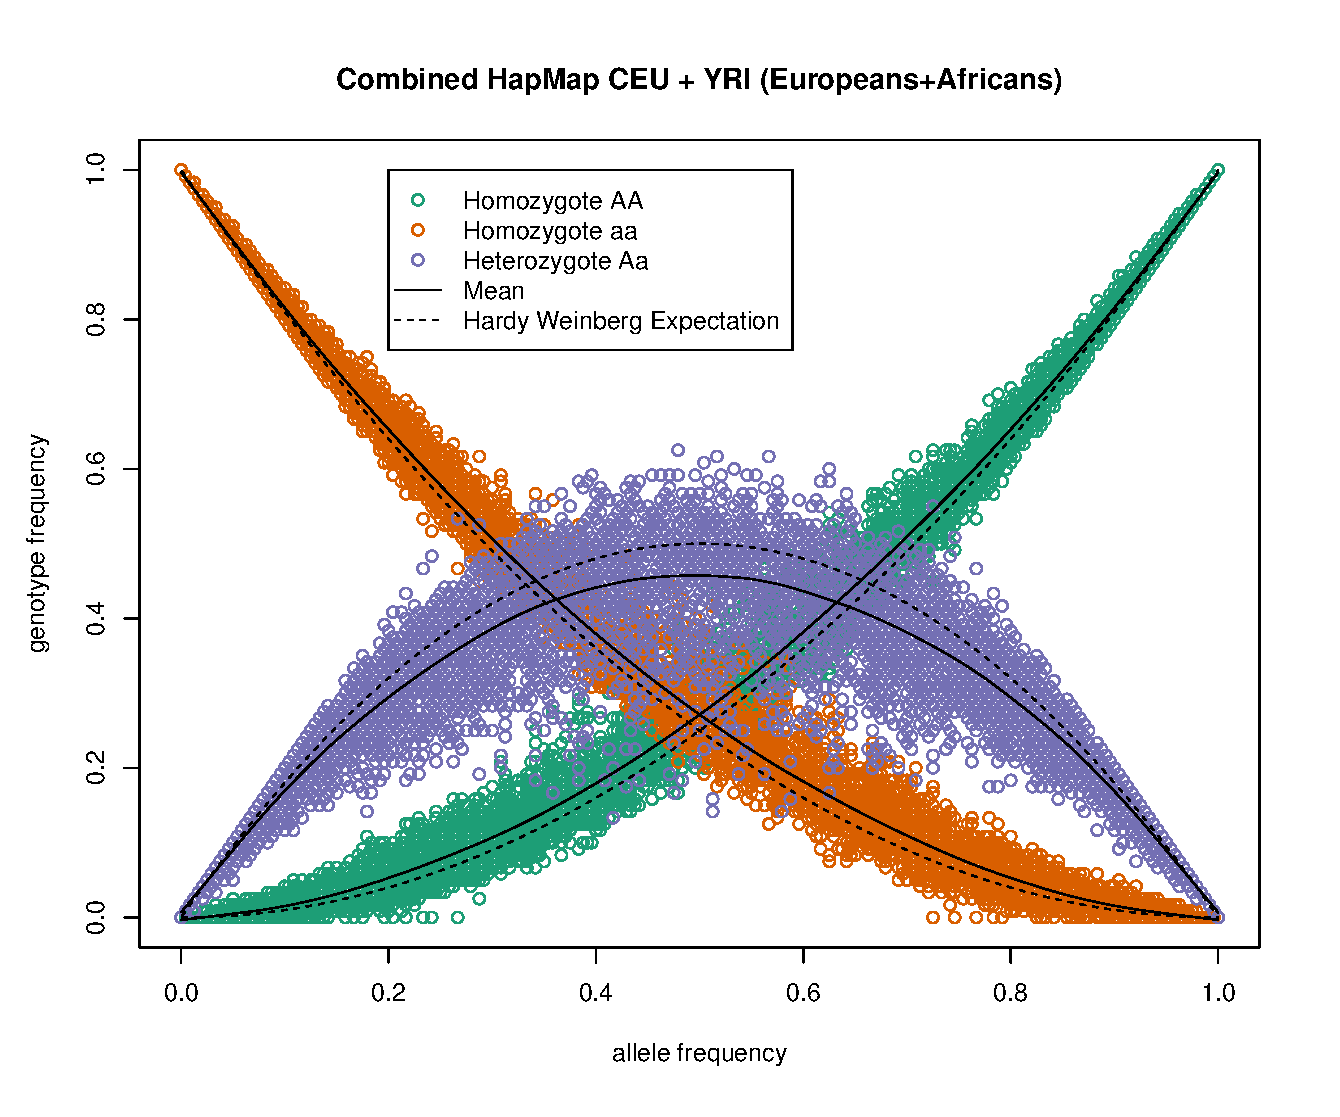
\includegraphics[width=0.5 \textwidth]{figures/CEU_YRI_together_HWE.eps}
\end{center}
\end{figure}


%figure/QT1.eps


\subsection{Coefficient of kinship}
We will define two alleles to be identical by descent if they are
identical due to a common ancestor in the past few generations. For the moment, we ignore mutation, and we will be more precise about what we mean by `past few generations' later on. For example, parent and child share exactly
one allele identical by descent at a locus, assuming that the two
parents of the child are randomly mated individuals from the population.\\

A key quantity is the probability that our pair of individuals share
0, 1, or 2 alleles identical by descent. We denote these probabilities
by $r_0$, $r_1$, and $r_2$ respectively. See Table \ref{table:IBDprobs} for
some examples. \\

One summary of relatedness that will be important is the probability that two alleles picked at random, one from each of the two different individuals $i$ and $j$, are identical by descent. We call this quantity the coefficient of kinship of individuals $i$ and $j$, and denote it by $F_{ij}$. It is calculated as
\begin{equation}
F_{ij}= 0 \times r_0 + \frac{1}{4} r_1  + \frac{1}{2} r_2. 
\label{eqn:coeffkinship}
\end{equation}

The coefficient of kinship will appear multiple times, in both our discussion of
inbreeding and in the context of phenotypic resemblance between relatives.\\

\begin{table}
\begin{center}
\begin{tabular}{| l | c c c c|}
\hline
Relationship (i,j)$^{*}$ & $r_0$ & $r_1$ & $r_2$ & $F_{ij}$\\
\hline
parent--child & 0 & 1 & 0 & 1/4\\
full siblings & 1/4 & 1/2 & 1/4 & 1/4\\
identical (monzygotic) twins  & 0 & 0 & 1  & 1/2 \\
$1^{st}$ cousins & 3/4 & 1/4 & 0 & 1/16\\
\hline
\end{tabular}
\end{center}
\caption{Probability that two individuals of a given relationship share 0, 1, or 2 alleles
identical by descent. $^{*}$ assuming this is the only relationship
the pair of individuals share (above that expected from randomly
sampling individuals from the population). } \label{table:IBDprobs}
\end{table}

\subsection{Inbreeding}
We can define an inbred individual as an individual whose parents are
more closely related to each other than two random individuals drawn
from some reference population.  \\

When two related individuals produce an offspring, that individual can
receive two alleles that are identical by descent, i.e.\ they
can be homozygous by descent (sometimes termed autozygous), due to the
fact that they have two copies of an allele through different paths
through the pedigree.  This increased likelihood of being homozygous
relative to an outbred individual is the most obvious effect of
inbreeding. It is also the one that will be of most interest to us, as it
underlies a lot of our ideas about inbreeding depression and
population structure.\\


As the offspring receives a random allele from each parent ($i$ and $j$), the
probability that those two alleles are identical by descent is equal to the
kinship coefficient $F_{ij}$ of the two parents (Eqn.\ \ref{eqn:coeffkinship}). This follows from the fact that
the genotype of the offspring is made by sampling an allele at random from each
of our parents. We will use IBD for identical by descent. \\

The only way the offspring can be heterozygous ($A_1 A_2$) is if their two alleles at a
locus are not IBD (otherwise they would necessarily be homozygous). Therefore, the probability that they are
heterozygous is
\begin{equation}
(1-F) 2p q,
\label{eq:hetGenHW}
\end{equation}
where we have dropped the indices $i$ and $j$ for simplicity.
The offspring can be homozygous for the $A_1$ allele in two different ways. 
They can have two non-IBD alleles that are not IBD but happen to be of the allelic type $A_1$,
or their two alleles can be IBD, such that they inherited allele $A_1$ by
two different routes from the same ancestor. Thus, the probability that an offspring is homozygous is
\begin{equation}
(1-F) p^2 + F p.
\end{equation}
Therefore, the frequencies of the three possible genotypes can be written as given in
Table \ref{table:GeneralizedHWE}, which provides a generalization of the Hardy--Weinberg
proportions.\\

\begin{table}
\begin{center}
\begin{tabular}{|ccc|}
\hline
$f_{11}$ & $f_{12}$ & $f_{22}$ \\
\hline
$(1-F) p^2 + F p$ & $(1-F) 2pq$ & $(1-F) q^2 + F q$ \\
\hline
\end{tabular}
\end{center}
\caption{\textbf{Generalized Hardy--Weinberg}} \label{table:GeneralizedHWE}
\end{table}

Note that the generalized Hardy--Weinberg proportions completely
specify the genotype probabilities, as there are two parameters ($p$ and $F$)
and two degrees of freedom (as $p$ and $q$ have to sum to one).
Therefore, any combination of genotype frequencies at a biallelic site
can be specified by a combination of $p$ and $F$.\\


\subsection{Calculating inbreeding coefficients from data}
If the observed heterozygosity in a population is $H_O$, and we assume that the generalized Hardy--Weinberg proportions hold, we can set $H_O$ equal to $f_{12}$, and solve Eq.\ \eqref{eq:hetGenHW} for $F$ to obtain an estimate of the inbreeding coefficient as
\begin{equation}
\hat{F} = 1-\frac{f_{12}}{2pq} = \frac{2pq - f_{12}}{2pq}.
\label{eqn:Fhat}
\end{equation}
As before, $p$ is the frequency of allele $A_{1}$ in the
population. This can be rewritten in terms of the observed heterozygosity ($H_O$)
and the heterozygosity expected in the absence of inbreeding, $H_E=2pq$, as
\begin{equation}
\hat{F} = \frac{H_E-H_O}{H_E} = 1 - \frac{H_O}{H_E}.
\label{eqn:FhatHO}
\end{equation}
Hence, $F$ quantifies the deviation due to inbreeding of the observed heterozygosity from the one expected under random mating, relative to the latter.
If we have multiple loci, we can replace $H_O$ and $H_E$ by their means
over loci, $\bar{H}_O$ and $\bar{H}_E$, respectively. Note that, in principle, we could also calculate $F$ for each individual locus first, and then take the average across loci. However, this procedure is more prone to introducing a bias if sample sizes vary across loci, which is not unlikely when we are dealing with real data.\\

%==Phenotypic resemblance between relatives ==
%<source-file filename="Quantative_traits.tex" display="Quantative_traits.wrapped.latexml.xhtml">

%==Phenotypic resemblance between relatives ==
%<source-file filename="Quantative_traits.tex" display="Quantative_traits.wrapped.latexml.xhtml">


\subsection{Summarizing population structure}
We defined inbreeding as having parents that are
more closely related to each other than two individuals drawn at random from some reference population. The question that naturally arises is: Which reference population should we use? While I might not look inbred in
comparison to allele frequencies in the United Kingdom (UK), where I am from, my
parents certainly are not two individuals drawn at random from the
world-wide population. If we estimated my inbreeding coefficient $F$ using allele frequencies
within the UK, it would 
be close to zero, but would likely be larger if we used world-wide
frequencies. This is because there is a somewhat lower level of
expected heterozygosity within the UK than in the human population across the world as a whole.\\

Wright (1943, 1951) developed a set of `F-statistics' (also called `fixation indices') that formalize the idea
of inbreeding with respect to different levels of population structure. He defined $F_{\mathrm{XY}}$ as
the correlation between random gametes, drawn from the same level $X$,
relative to level $Y$. We will return to why $F$-statistics are statements
about correlations between alleles in just a moment. One commonly uses $\fis$ for the inbreeding
coefficient between an individual ($I$) and the subpopulation
($S$). Consider a single locus, where in a subpopulation ($S$) a fraction $H_I=f_{12}$ of individuals
are heterozygous. In this subpopulation, let the frequency of
allele $A_1$ be $p_S$, such that the expected heterozygosity under random mating is $H_S = 2 p_S (1 - p_S)$. We will write $\fis$ as
\begin{equation}
\fis = 1-\frac{H_I}{H_S}= 1-\frac{f_{12}}{2p_Sq_S},
\label{eqn:FIS}
\end{equation}
a direct analog of eqn. \ref{eqn:Fhat}. Hence, $\fis$ is the relative difference between observed and expected heterozygosity due to a deviation from random mating within the subpopulation. We could also compare the observed
heterozygosity in individuals ($H_I$) to that expected in the total
population, $H_T$. If the frequency of allele $A_1$ in the total
population is $p_T$, then we can write $\fit$ as
\begin{equation}
\fit =1-\frac{H_I}{H_T}= 1-\frac{f_{12}}{2p_Tq_T},
\label{eqn:FIT}
\end{equation}
which compares heterozygosity in individuals to that expected in the
total population. As a simple extension of this, we could imagine
comparing the expected heterozygosity in the subpopulation ($H_S$) to
that expected in the total population $H_T$, via $\fst$:
\begin{equation}
\fst = 1-\frac{H_S}{H_T}=1-\frac{2p_Sq_S}{2p_Tq_T} \label{eqn:FST}.
\end{equation}
If the total population contains the subpopulation then, as we will see
below, due to the Wahlund effect (to be added)
 $2p_Sq_S \leq
2p_Tq_T$, and so $\fis \leq \fit$ and $\fst \geq 0$. We can
relate the three $F$-statistics to each other as
\begin{equation}
(1-\hat{\fit}) =\frac{H_I}{H_S} \frac{H_S}{H_T}=(1-\fis)(1-\fst).
\label{eqn:F_relationships}
\end{equation}
Hence, the reduction in heterozygosity within individuals compared to that expected
in the total population can be decomposed to the reduction in
heterozygosity of individuals compared to the subpopulation, and the reduction in
heterozygosity from the total population to that in the subpopulation.\\

If we want a summary of
population structure across multiple subpopulations, we can average $H_I$
and/or $H_S$ across populations, and use a $p_T$ calculated by
averaging $p_S$ across subpopulations (or our samples from sub-populations). For example, the average $\fst$ across $K$ subpopulations (sampled with equal effort) is
\begin{equation}
	\fst = 1 - \frac{\bar{H}_{S}}{H_T},
\end{equation}
where $\bar{H}_S = 1/K \sum_{i = 1}^{K} H_{S}^{(i)}$, and $H_{S}^{(i)} = 2 p_{i} q_{i}$ is the expected heterozygosity in subpopulation $i$.
Furthermore, if we have multiple sites, we can replace $H_I$, $H_S$, and $H_T$ with their averages across loci (as above). \\

Let us now return to Wright's definition of the $F$-statistics as correlations between random gametes, drawn from the same level $X$,
relative to level $Y$. Without loss of generality, we may think about $X$ as
individuals and $S$ as the subpopulation.
Rewriting $\fis$ in terms of the observed homozygote frequencies ($f_{11}$, $f_{22}$) and expected homozygosities ($p_{S}^2$, $q_{S}^2$) we find
\begin{equation}
\fis = \frac{2p_Sq_S - f_{12}}{2p_Sq_S} = \frac{f_{11}+f_{22} -
p_S^2 - q_S^2}{2p_Sq_S},
\label{eqn:Fascorr}
\end{equation}
using the fact that $p^2+2pq+q^2=1$, and $f_{12} = 1 - f_{11} - f_{12}$. The form of eqn.\ (\ref{eqn:Fascorr}) reveals that $\fis$ is the covariance between pairs of alleles
found in an individual, divided by the
expected variance under binomial sampling. Thus, $F$-statistics can be
understood as the correlation between alleles drawn from a population
(or an individual) above that expected by chance (i.e.\ drawing alleles
sampled at random from some broader population).\\

We can also interpret $F$-statistics as proportions of variance explained by
different levels of population structure. To see this, let us think about $\fst$ averaged over $K$
subpopulations, whose frequencies are $p_1,\dots,p_K$. The
frequency in the total population is $p_T=\bar{p} = 1/K \sum_{i=1}^K p_i$.
Then, we can
write
\begin{equation}
\fst = \frac{2 \bar{p}\bar{q} - \frac{1}{K}\sum_{i=1}^K 2p_iq_i }{2
\bar{p}\bar{q}} = \frac{ \left(\frac{1}{K} \sum_{i=1}^K p_i^2 +
\frac{1}{K} \sum_{i=1}^K q_i^2 \right) -  \bar{p}^2-\bar{q}^2 }{2
\bar{p}\bar{q}} = \frac{\mathrm{Var}(p_i)}{\mathrm{Var}(\bar{p})},
\label{eqn:F_as_propvar}
\end{equation}
which shows that $\fst$ is the proportion of the variance explained by the
subpopulation labels.


\newpage
